% Template per generare

\documentclass[a4paper,11pt]{article}
\usepackage{lmodern}
\renewcommand*\familydefault{\sfdefault}
\usepackage{sfmath}
\usepackage[utf8]{inputenc}
\usepackage[T1]{fontenc}
\usepackage[italian]{babel}
\usepackage{indentfirst}
\usepackage{graphicx}
\usepackage{tikz}
\newcommand*\circled[1]{\tikz[baseline=(char.base)]{
		\node[shape=circle,draw,inner sep=2pt] (char) {#1};}}
\usepackage{enumitem}
% \usepackage[group-separator={\,}]{siunitx}
\usepackage[left=2cm, right=2cm, bottom=3cm]{geometry}
\frenchspacing

\newcommand{\num}[1]{#1}

% Macro varie...
\newcommand{\file}[1]{\texttt{#1}}
\renewcommand{\arraystretch}{1.3}
\newcommand{\esempio}[2]{
\noindent\begin{minipage}{\textwidth}
\begin{tabular}{|p{11cm}|p{5cm}|}
	\hline
	\textbf{File \file{input.txt}} & \textbf{File \file{output.txt}}\\
	\hline
	\tt \small #1 &
	\tt \small #2 \\
	\hline
\end{tabular}
\end{minipage}
}

% Dati del task
\newcommand{\gara}{Olimpiadi Italiane di Informatica - Selezioni Territoriali 2013}
\newcommand{\nome}{A spasso per Brisbane}
\newcommand{\nomebreve}{brisbane}

\begin{document}


% Intestazione
\noindent{\Large \gara}
\vspace{0.5cm}

\noindent{\Huge \textbf \nome~(\texttt{\nomebreve})}
\vspace{0.2cm}\\
\noindent{\large \textsc{Difficoltà D=2}}

% Descrizione del task
\section*{Descrizione del problema}
Nel 2013, le IOI si svolgeranno a Brisbane (in Australia).  La
rappresentativa italiana ha già iniziato a studiare la città, per
capire cosa ci sia di interessante da vedere, e come ci si possa
spostare nella giornata libera successiva alla seconda gara delle
Olimpiadi.

L'offerta di trasporto pubblico a Brisbane è abbastanza variegata: ci
sono due linee di bus, di cui una gratuita che gira intorno alla
città, e due linee di traghetti che fermano in diversi punti del fiume
Brisbane, che taglia la città in due; per quello che riguarda i
prezzi, esiste un abbonamento giornaliero a tutti i trasporti
pubblici, bus e traghetti insieme, oppure è possibile prendere un più
economico abbonamento giornaliero ai soli traghetti, o un ancor più
economico abbonamento ai soli bus.

La squadra italiana vorrà visitare il maggior numero di attrazioni
possibile e per questo motivo Monica, la responsabile
dell’organizzazione, ha deciso di cercare un buon compromesso tra il
prezzo dei biglietti e le attrazioni che sarà possibile raggiungere
partendo dall’hotel.

Data una lista di attrazioni e la mappa dei collegamenti delle diverse
linee del trasporto pubblico, il vostro compito è quello di aiutare
Monica a capire \emph{quante attrazioni sono raggiungibili} per ogni
possibile scelta dei biglietti per i trasporti pubblici.

\begin{center}
  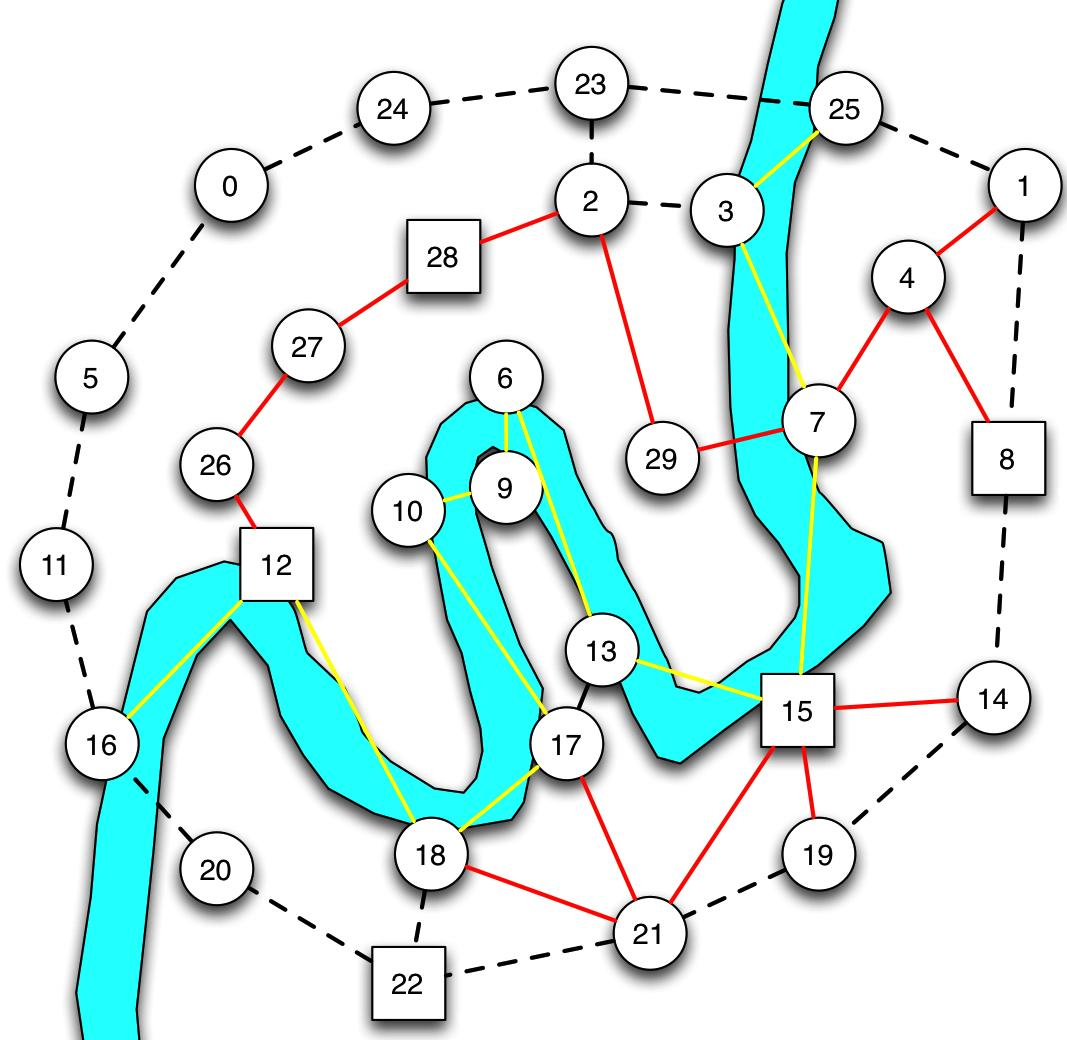
\includegraphics[width=8cm]{image01.jpg}
\end{center}

Per esempio, possiamo fare riferimento alla figura qui sopra, dove ad
ogni fermata è associato un \emph{cerchio} (o un \emph{quadrato} nel
caso di luogo di attrazione) e i collegamenti sono:

\begin{itemize}[nolistsep, noitemsep]
  \item tratteggiati -- collegamenti gratuiti (bus gratuiti e brevi
    percorsi a piedi);
  \item rossi -- bus a pagamento;
  \item gialli -- traghetto.
\end{itemize}

\noindent
Il punto di partenza della rappresentativa italiana è la fermata
numero $0$; le attrazioni da vedere sono quelle rappresentate con un
quadrato, numerate rispettivamente $8$, $12$, $15$, $22$ e $28$.  Come
si può vedere, spostandosi con i mezzi gratuiti si raggiungono solo
due attrazioni (la numero $8$ e la numero $22$); comprando il
biglietto del bus si raggiungono tutte le attrazioni; comprando il
biglietto del traghetto si raggiungono, oltre alla $8$ e la $22$,
anche la $12$ e la $15$ per un totale di quattro attrazioni. Il
biglietto combinato, in questo caso, raggiunge tutte le attrazioni.

\section*{Dati di input}
Il file \verb'input.txt' è composto da $1+A+M_G+M_B+M_T$ righe. La
prima riga contiene cinque interi positivi separati da uno spazio, che
rappresentano il numero $N$ delle fermate, il numero $A$ di
attrazioni, il numero $M_G$ dei collegamenti gratuiti, il numero $M_B$
dei collegamenti via bus e il numero $M_T$ dei collegamenti via
traghetto.  Ogni fermata è rappresentata da un intero compreso tra $0$
e $N-1$.  Le successive $A$ righe contengono ognuna una fermata (un
intero compreso tra $0$ e $N-1$) corrispondente ad una delle
attrazioni che la rappresentativa italiana può visitare.  Ognuna delle
successive $M_G+M_B+M_T$ righe contiene un collegamento del trasporto
pubblico, rappresentato da due interi positivi: le fermate collegate.
Le prime $M_G$ righe contengono i collegamenti gratuiti (bus gratuiti
e brevi percorsi a piedi), poi le successive $M_B$ contengono i
collegamenti del bus a pagamento e infine le ultime $M_T$ righe
contengono i collegamenti dei traghetti.  Il punto di partenza della
rappresentativa italiana è la sempre la fermata numero $0$.

\section*{Dati di output}
Il file \verb'output.txt' è composto da $4$ righe contenenti ognuna un
intero non negativo, rispettivamente, il numero di attrazioni
raggiungibili:
\begin{enumerate}[nolistsep, noitemsep]
  \item senza comprare biglietti (solo con mezzi gratis);
  \item comprando solo il biglietto giornaliero dei bus;
  \item comprando solo il biglietto giornaliero dei traghetti;
  \item comprando entrambe le tipologie di biglietti.
\end{enumerate}

% Assunzioni
\section*{Assunzioni}
\begin{itemize}[nolistsep, noitemsep]
  \item $2 \le N \le 1000$
  \item $N \le M_G+M_B+M_T \le 10\,000$
\end{itemize}

% Esempi
\section*{Esempio di input/output}
\esempio{
6 2 2 4 2

1

5

0 1

2 5

0 3

1 3

2 4

4 5

1 2

3 4
}{
1

1

2

2
}

\esempio{
30 5 18 14 11

8

12

15

22

28

0 5

0 24

1 8

1 25

2 3

2 23

5 11

8 14

11 16

13 17

14 19

16 20

18 22

19 21

20 22

21 22

23 24

23 25

1 4

2 28

2 29

4 7

4 8

7 29

12 26

14 15

15 19

15 21

17 21

18 21

26 27

27 28

3 7

3 25

6 9

6 13

7 15

9 10

10 17

12 16

12 18

13 15

17 18
}{
2

5

4

5
}

\section*{Note}
\begin{itemize}
  \item Il secondo caso di esempio corrisponde alla situazione presentata in figura.
  \item Un programma che restituisce sempre lo stesso valore, indipendentemente dai dati in \texttt{input.txt}, non totalizza alcun punteggio.
\end{itemize}

\end{document}
